% Created 2026-04-22 Wed 18:21
% Intended LaTeX compiler: pdflatex
\documentclass{article}
\usepackage[utf8]{inputenc}
\usepackage[T1]{fontenc}
\usepackage{graphicx}
\usepackage{longtable}
\usepackage{wrapfig}
\usepackage{rotating}
\usepackage[normalem]{ulem}
\usepackage{amsmath}
\usepackage{amssymb}
\usepackage{capt-of}
\usepackage{hyperref}

\usepackage{fancyhdr}
\usepackage[top=25mm, left=25mm, right=25mm]{geometry}
\usepackage{longtable}
\fancyhead[R]{}
\setlength\headheight{43.0pt}
\usepackage{tabularx}
\usepackage{longtable}
\author{A-EVAN MATANGO B-EDGAR ENDARA D-KAREN SUAREZ}
\date{2026-04-08}
\title{Taller de Configuracion de Entorno WSL}
\hypersetup{
 pdfauthor={A-EVAN MATANGO B-EDGAR ENDARA D-KAREN SUAREZ},
 pdftitle={Taller de Configuracion de Entorno WSL},
 pdfkeywords={},
 pdfsubject={},
 pdfcreator={Emacs 27.1 (Org mode 9.7.5)}, 
 pdflang={Espanol}}
\begin{document}

\maketitle
\fancyhead[C]{\includegraphics[scale=0.05]{../images/logoEPN.jpg}\\
ESCUELA POLITECNICA NACIONAL\\FACULTAD DE INGENIERIA DE SISTEMAS\\
ARQUITECTURA DE COMPUTADORES}
\thispagestyle{fancy}

\section{Objetivos}
\label{sec:org6370855}

\begin{itemize}
\item Configurar y validar el entorno de trabajo para la asignatura de Arquitectura de Computadores en Linux o WSL.
\item Verificar la instalacion de herramientas base: mamba/anaconda (Python), Emacs y \LaTeX.
\item Documentar evidencias tecnicas mediante capturas y comandos ejecutados.
\end{itemize}

\section{Instrucciones}
\label{sec:org94a55c2}

\begin{enumerate}
\item Realice todas las actividades en Linux o en WSL.
\item En cada sección ejecute los comandos solicitados y registre la salida en el bloque correspondiente.
\item Guarde el archivo y exporte a pdf con el comando `org-latex-export-to-pdf`.
\item Verifique que estén todos los nombres de los integrantes del grupo
de trabajo. Los grupos para este trabajo están en \href{https://epnecuador.sharepoint.com/:x:/s/ICCD332-ArquitecturaComputadores/IQCjNuELSDbJTb42EfrLL2ksATBSbitbZ9\_iFLJxIiCtSr0?e=gowv5I}{Equipos de Trabajo}.
\item Verifique que en las distintas secciones de este archivo esté
identificado con nombre e email el aporte del estudiante.
\end{enumerate}

Si require insertar una imagen, crear una carpeta \texttt{images} y colocar
la imagen dentro. Para llamar la imagen desde Emacs use \texttt{C-c C-l} y
busque el archivo o escriba:Puede insertar una imagen con la sintaxis:

\begin{verbatim}
[[./images/image1.jpg]]
\end{verbatim}
\section{Actividades}
\label{sec:org93923b8}
\subsection{Configuración de WSL con Ubuntu, \LaTeX, Python e Emacs}
\label{sec:orgcd3c01e}

\begin{enumerate}
\item Verificacion de entorno mamba/anaconda
\begin{enumerate}
\item Active WSL (si aplica) y su entorno de trabajo.
\item Ejecute \texttt{mamba info} con \texttt{C-c C-c} dentro del bloque de código.
\item Si el comando falla, active un entorno con \texttt{mamba activate
      iccd332} e intente de nuevo.
\end{enumerate}
\end{enumerate}


\subsubsection{Estudiante: Evan}
\label{sec:org5b69326}

\begin{verbatim}
     mamba info
\end{verbatim}
\begin{verbatim}

	  libmamba version : 2.5.0
	     mamba version : 2.5.0
	      curl version : libcurl/8.19.0 OpenSSL/3.6.1 zlib/1.3.2 zstd/1.5.7 libssh2/1.11.1 nghttp2/1.68.1 mit-krb5/1.22.2
	libarchive version : libarchive 3.8.6 zlib/1.3.2 liblzma/5.8.2 bz2lib/1.0.8 liblz4/1.10.0 libzstd/1.5.7 liblzo2/2.10 openssl/3.5.5 libb2/bundled
	  envs directories : /home/evanmh-epn/miniforge3/envs
	     package cache : /home/evanmh-epn/miniforge3/pkgs
			     /home/evanmh-epn/.mamba/pkgs
	       environment : iccd332 (active)
	      env location : /home/evanmh-epn/miniforge3/envs/iccd332
	 user config files : /home/evanmh-epn/.mambarc
    populated config files : /home/evanmh-epn/miniforge3/.condarc
	  virtual packages : __unix=0=0
			     __linux=6.6.87=0
			     __glibc=2.39=0
			     __archspec=1=x86_64_v3
			     __cuda=12.7=0
		  channels : https://conda.anaconda.org/conda-forge/linux-64
			     https://conda.anaconda.org/conda-forge/noarch
	  base environment : /home/evanmh-epn/miniforge3
		  platform : linux-64
\end{verbatim}


\subsubsection{Estudiante:Endara Sebastian}
\label{sec:org0b29b13}
\begin{verbatim}
     mamba info
\end{verbatim}

\begin{verbatim}

	  libmamba version : 2.5.0
	     mamba version : 2.5.0
	      curl version : libcurl/8.19.0 OpenSSL/3.6.1 zlib/1.3.2 zstd/1.5.7 libssh2/1.11.1 nghttp2/1.68.1 mit-krb5/1.22.2
	libarchive version : libarchive 3.8.6 zlib/1.3.2 liblzma/5.8.2 bz2lib/1.0.8 liblz4/1.10.0 libzstd/1.5.7 liblzo2/2.10 openssl/3.5.5 libb2/bundled
	  envs directories : /home/evanmh-epn/miniforge3/envs
	     package cache : /home/evanmh-epn/miniforge3/pkgs
			     /home/evanmh-epn/.mamba/pkgs
	       environment : iccd332 (active)
	      env location : /home/evanmh-epn/miniforge3/envs/iccd332
	 user config files : /home/evanmh-epn/.mambarc
    populated config files : /home/evanmh-epn/miniforge3/.condarc
	  virtual packages : __unix=0=0
			     __linux=6.6.87=0
			     __glibc=2.39=0
			     __archspec=1=x86_64_v3
			     __cuda=12.7=0
		  channels : https://conda.anaconda.org/conda-forge/linux-64
			     https://conda.anaconda.org/conda-forge/noarch
	  base environment : /home/evanmh-epn/miniforge3
		  platform : linux-64
\end{verbatim}


\subsubsection{Estudiante:Joset Muela}
\label{sec:org3b200a0}
\begin{verbatim}
     mamba info
\end{verbatim}

\begin{verbatim}

	  libmamba version : 2.5.0
	     mamba version : 2.5.0
	      curl version : libcurl/8.19.0 OpenSSL/3.6.1 zlib/1.3.2 zstd/1.5.7 libssh2/1.11.1 nghttp2/1.68.1 mit-krb5/1.22.2
	libarchive version : libarchive 3.8.6 zlib/1.3.2 liblzma/5.8.2 bz2lib/1.0.8 liblz4/1.10.0 libzstd/1.5.7 liblzo2/2.10 openssl/3.5.5 libb2/bundled
	  envs directories : /home/evanmh-epn/miniforge3/envs
	     package cache : /home/evanmh-epn/miniforge3/pkgs
			     /home/evanmh-epn/.mamba/pkgs
	       environment : iccd332 (active)
	      env location : /home/evanmh-epn/miniforge3/envs/iccd332
	 user config files : /home/evanmh-epn/.mambarc
    populated config files : /home/evanmh-epn/miniforge3/.condarc
	  virtual packages : __unix=0=0
			     __linux=6.6.87=0
			     __glibc=2.39=0
			     __archspec=1=x86_64_v3
			     __cuda=12.7=0
		  channels : https://conda.anaconda.org/conda-forge/linux-64
			     https://conda.anaconda.org/conda-forge/noarch
	  base environment : /home/evanmh-epn/miniforge3
		  platform : linux-64
\end{verbatim}


\subsubsection{Estudiante: Karen Suarez}
\label{sec:org203fde9}

\begin{verbatim}
     mamba info
\end{verbatim}

\begin{verbatim}

	  libmamba version : 2.5.0
	     mamba version : 2.5.0
	      curl version : libcurl/8.19.0 OpenSSL/3.6.1 zlib/1.3.2 zstd/1.5.7 libssh2/1.11.1 nghttp2/1.68.1 mit-krb5/1.22.2
	libarchive version : libarchive 3.8.6 zlib/1.3.2 liblzma/5.8.2 bz2lib/1.0.8 liblz4/1.10.0 libzstd/1.5.7 liblzo2/2.10 openssl/3.5.5 libb2/bundled
	  envs directories : /home/evanmh-epn/miniforge3/envs
	     package cache : /home/evanmh-epn/miniforge3/pkgs
			     /home/evanmh-epn/.mamba/pkgs
	       environment : iccd332 (active)
	      env location : /home/evanmh-epn/miniforge3/envs/iccd332
	 user config files : /home/evanmh-epn/.mambarc
    populated config files : /home/evanmh-epn/miniforge3/.condarc
	  virtual packages : __unix=0=0
			     __linux=6.6.87=0
			     __glibc=2.39=0
			     __archspec=1=x86_64_v3
			     __cuda=12.7=0
		  channels : https://conda.anaconda.org/conda-forge/linux-64
			     https://conda.anaconda.org/conda-forge/noarch
	  base environment : /home/evanmh-epn/miniforge3
		  platform : linux-64
\end{verbatim}

\begin{enumerate}
\item Verificacion de Python
\begin{enumerate}
\item Active el entorno \texttt{iccd332} para abrir Emacs con \texttt{mamba activate iccd332}.
\item Ejecute \texttt{python -{}-{}version} en la consola y desde Emacs.
\end{enumerate}
\end{enumerate}


\subsubsection{Estudiante Evan:}
\label{sec:org20dd320}
\begin{verbatim}
    python --version
\end{verbatim}

\begin{verbatim}
Python 3.14.4
\end{verbatim}

\subsubsection{Estudiante Edgar Endara:}
\label{sec:org13f4550}
\begin{verbatim}
    python --version
\end{verbatim}

\begin{verbatim}
Python 3.14.4
\end{verbatim}


\subsubsection{Estudiante :Joset Muela}
\label{sec:org2e91795}
\begin{verbatim}
    python --version
\end{verbatim}

\begin{verbatim}
Python 3.14.4
\end{verbatim}

\subsubsection{Estudiante Karen Suarez:}
\label{sec:org6191121}
\begin{verbatim}
    python --version
\end{verbatim}

\begin{verbatim}
Python 3.14.4
\end{verbatim}


\#+RESULTS
\begin{verbatim}
Python 3.14.4
\end{verbatim}



\begin{enumerate}
\item Verificacion de Emacs
Ejecute \texttt{emacs -{}-{}version} en la consola y desde Emacs.
\end{enumerate}


\subsubsection{Estudiante Evan Matango:}
\label{sec:orgecbf543}
\begin{verbatim}
   emacs --version
\end{verbatim}

\begin{verbatim}
GNU Emacs 29.3
Copyright (C) 2024 Free Software Foundation, Inc.
GNU Emacs comes with ABSOLUTELY NO WARRANTY.
You may redistribute copies of GNU Emacs
under the terms of the GNU General Public License.
For more information about these matters, see the file named COPYING.
\end{verbatim}

\subsubsection{Estudiante Edgar Endara:}
\label{sec:org2f867a7}
\begin{verbatim}
   emacs --version
\end{verbatim}

\begin{verbatim}
GNU Emacs 29.3
Copyright (C) 2024 Free Software Foundation, Inc.
GNU Emacs comes with ABSOLUTELY NO WARRANTY.
You may redistribute copies of GNU Emacs
under the terms of the GNU General Public License.
For more information about these matters, see the file named COPYING.
\end{verbatim}

\subsubsection{Estudiante :Joset Muela}
\label{sec:orgb6240ad}
\begin{verbatim}
   emacs --version
\end{verbatim}

\begin{verbatim}
GNU Emacs 29.3
Copyright (C) 2024 Free Software Foundation, Inc.
GNU Emacs comes with ABSOLUTELY NO WARRANTY.
You may redistribute copies of GNU Emacs
under the terms of the GNU General Public License.
For more information about these matters, see the file named COPYING.
\end{verbatim}

\subsubsection{Estudiante Karen Suarez:}
\label{sec:org9b01267}

\begin{verbatim}
   emacs --version
\end{verbatim}

\begin{verbatim}
GNU Emacs 29.3
Copyright (C) 2024 Free Software Foundation, Inc.
GNU Emacs comes with ABSOLUTELY NO WARRANTY.
You may redistribute copies of GNU Emacs
under the terms of the GNU General Public License.
For more information about these matters, see the file named COPYING.
\end{verbatim}


\begin{enumerate}
\item Verificacion de \LaTeX{}
Ejecute \texttt{latex -{}-{}version} en la consola y desde Emacs.
\end{enumerate}

\subsubsection{Estudiante Evan Matango:}
\label{sec:org5006043}

\begin{verbatim}
   latex --version
\end{verbatim}

\begin{verbatim}
   pdfTeX 3.141592653-2.6-1.40.25 (TeX Live 2023/Debian)
   kpathsea version 6.3.5
   Copyright 2023 Han The Thanh (pdfTeX) et al.
   There is NO warranty.  Redistribution of this software is
   covered by the terms of both the pdfTeX copyright and
   the Lesser GNU General Public License.
   For more information about these matters, see the file
   named COPYING and the pdfTeX source.
   Primary author of pdfTeX: Han The Thanh (pdfTeX) et al.
   Compiled with libpng 1.6.43; using libpng 1.6.43
   Compiled with zlib 1.3; using zlib 1.3
   Compiled with xpdf version 4.04
\end{verbatim}

\subsubsection{Estudiante Endara Sebastian:}
\label{sec:orga89f9b3}

\begin{verbatim}
   latex --version
\end{verbatim}

\begin{verbatim}
   pdfTeX 3.141592653-2.6-1.40.25 (TeX Live 2023/Debian)
   kpathsea version 6.3.5
   Copyright 2023 Han The Thanh (pdfTeX) et al.
   There is NO warranty.  Redistribution of this software is
   covered by the terms of both the pdfTeX copyright and
   the Lesser GNU General Public License.
   For more information about these matters, see the file
   named COPYING and the pdfTeX source.
   Primary author of pdfTeX: Han The Thanh (pdfTeX) et al.
   Compiled with libpng 1.6.43; using libpng 1.6.43
   Compiled with zlib 1.3; using zlib 1.3
   Compiled with xpdf version 4.04
\end{verbatim}

\subsubsection{Estudiante :Joset Muela}
\label{sec:org66d2d20}

\begin{verbatim}
   latex --version
\end{verbatim}

\begin{verbatim}
   pdfTeX 3.141592653-2.6-1.40.25 (TeX Live 2023/Debian)
   kpathsea version 6.3.5
   Copyright 2023 Han The Thanh (pdfTeX) et al.
   There is NO warranty.  Redistribution of this software is
   covered by the terms of both the pdfTeX copyright and
   the Lesser GNU General Public License.
   For more information about these matters, see the file
   named COPYING and the pdfTeX source.
   Primary author of pdfTeX: Han The Thanh (pdfTeX) et al.
   Compiled with libpng 1.6.43; using libpng 1.6.43
   Compiled with zlib 1.3; using zlib 1.3
   Compiled with xpdf version 4.04
\end{verbatim}

\subsubsection{Estudiante Karen Suarez:}
\label{sec:org449f078}

\begin{verbatim}
   latex --version
\end{verbatim}

\begin{verbatim}
   pdfTeX 3.141592653-2.6-1.40.25 (TeX Live 2023/Debian)
   kpathsea version 6.3.5
   Copyright 2023 Han The Thanh (pdfTeX) et al.
   There is NO warranty.  Redistribution of this software is
   covered by the terms of both the pdfTeX copyright and
   the Lesser GNU General Public License.
   For more information about these matters, see the file
   named COPYING and the pdfTeX source.
   Primary author of pdfTeX: Han The Thanh (pdfTeX) et al.
   Compiled with libpng 1.6.43; using libpng 1.6.43
   Compiled with zlib 1.3; using zlib 1.3
   Compiled with xpdf version 4.04
\end{verbatim}



\begin{enumerate}
\item Registro de problemas y solucion aplicada
\end{enumerate}

Complete la siguiente tabla si tuvo errores durante la configuración:

\begin{center}
\begin{tabularx}{\textwidth}{lXX}
\textbf{Herramienta} & \textbf{Problema observado} & \textbf{Solucion aplicada}\\[0pt]
\hline
 &  & \\[0pt]
 &  & \\[0pt]
 &  & \\[0pt]
\end{tabularx}
\end{center}

\subsection{Comandos Emacs Tutorial}
\label{sec:org625c8b2}
Seguir el tutorial integrado en Emacs al respecto de la navegación y
operaciones más frecuentes. El tutorial puede ser accedido en Español
utilizando el comando:

\begin{verbatim}
M-x help-with-tutorial-spec-language
\end{verbatim}

Realice los ejercicios del tutorial (al menos un 80\% del texto) y
complete la siguiente tabla con los comandos que considere de mayor
interés. Verifique que en la parte superior se active el menú de
tabla. Dentro de la región de la tabla puede dar C-c C-c para alinear
automáticamente la tabla al contenido del texto que escriba. Para
generar una nueva fila escriba presione la tecla TAB

<Estudiante A Evan Matango>
\begin{longtable}{|p{0.2\linewidth}|p{0.3\linewidth}|p{0.2\linewidth}|p{0.3\linewidth}|}
\textbf{Comando} & \textbf{Descripción} & \textbf{Comando} & \textbf{Descripción}\\[0pt]
\hline
\endfirsthead
\multicolumn{4}{l}{Continued from previous page} \\[0pt]
\hline

\textbf{Comando} & \textbf{Descripción} & \textbf{Comando} & \textbf{Descripción} \\[0pt]

\hline
\endhead
\hline\multicolumn{4}{r}{Continued on next page} \\
\endfoot
\endlastfoot
\hline
\texttt{C-c C-e \# latex} & Insertar template de  latex & \texttt{C-x C-s} & Guardar los cambios en el archivo\\[0pt]
\texttt{C-x k} & Matar un buffer & \texttt{C-/} & Deshace una acción\\[0pt]
\texttt{C-x 1} & Cerrar una ventana & \texttt{C-h k C-f} & Saber que hace un comando\\[0pt]
\texttt{C-x C-b} & Ver los buffers & \texttt{M-k} & Borrar una línea\\[0pt]
\end{longtable}

<Estudiante Edgar Endara>
\begin{longtable}{|p{0.2\linewidth}|p{0.3\linewidth}|p{0.2\linewidth}|p{0.3\linewidth}|}
\textbf{Comando} & \textbf{Descripción} & \textbf{Comando} & \textbf{Descripción}\\[0pt]
\hline
\endfirsthead
\multicolumn{4}{l}{Continued from previous page} \\[0pt]
\hline

\textbf{Comando} & \textbf{Descripción} & \textbf{Comando} & \textbf{Descripción} \\[0pt]

\hline
\endhead
\hline\multicolumn{4}{r}{Continued on next page} \\
\endfoot
\endlastfoot
\hline
\texttt{C-g} & Cancelar comando & \texttt{C-l} & Centrar cursosr en pantalla\\[0pt]
\texttt{C-x C-f} & Abrir archivo & \texttt{C-x u} & Deshacer\\[0pt]
\texttt{C-x C-t} & Transponer líneas & \texttt{M-w} & Copiar región\\[0pt]
\end{longtable}

<Estudiante Joset Muela>
\begin{longtable}{|p{0.2\linewidth}|p{0.3\linewidth}|p{0.2\linewidth}|p{0.3\linewidth}|}
\textbf{Comando} & \textbf{Descripción} & \textbf{Comando} & \textbf{Descripción}\\[0pt]
\hline
\endfirsthead
\multicolumn{4}{l}{Continued from previous page} \\[0pt]
\hline

\textbf{Comando} & \textbf{Descripción} & \textbf{Comando} & \textbf{Descripción} \\[0pt]

\hline
\endhead
\hline\multicolumn{4}{r}{Continued on next page} \\
\endfoot
\endlastfoot
\hline
\texttt{C-c C-e \# latex} & Insertar template de  latex & \texttt{C-x C-s} & Guardar los cambios en el archivo\\[0pt]
\texttt{C-g} & Cancelar comando & \texttt{C-x u} & Deshace una acción\\[0pt]
\texttt{C-x C-b} & Lista de buffers & \texttt{C-x b} & Cambiar a otro buffer\\[0pt]
\texttt{C-x C-f} & Encontrar un archivo & \texttt{C-x 1} & Borrar todo menos una ventana\\[0pt]
\end{longtable}

<Estudiante D Karen Suarez >
\begin{longtable}{|p{0.2\linewidth}|p{0.3\linewidth}|p{0.2\linewidth}|p{0.3\linewidth}|}
\textbf{Comando} & \textbf{Descripción} & \textbf{Comando} & \textbf{Descripción}\\[0pt]
\hline
\endfirsthead
\multicolumn{4}{l}{Continued from previous page} \\[0pt]
\hline

\textbf{Comando} & \textbf{Descripción} & \textbf{Comando} & \textbf{Descripción} \\[0pt]

\hline
\endhead
\hline\multicolumn{4}{r}{Continued on next page} \\
\endfoot
\endlastfoot
\hline
\texttt{C-c C-e \# latex} & Insertar template de  latex & \texttt{C-x C-s} & Guardar los cambios en el archivo\\[0pt]
\texttt{C-x r SPC \#Registros y Bookmarks} & Guardar posición en registro & \texttt{C-x 1} & Para abrir todo el texto en una sola ventana\\[0pt]
\texttt{C-d \#Insertar y borrar} & Borra el caracter que esta despues del cursor & \texttt{C-x C-f} & Para encontrar el archivo\\[0pt]
\texttt{C-x C-b \#buffers} & Ayuda a ver la lista de buffers & \texttt{C-x 2} & Ayuda a separar la pantalla en dos ventanas\\[0pt]
\end{longtable}
\subsection{Comandos Emacs Juego}
\label{sec:orgccb4129}
En la anterior sección usted revisó los comandos de mayor interés
sobre la manipulación de Emacs. Es hora de poner en práctica sus
conocimientos. Realice unas 3 visitas al juego  \href{https://chat.qwen.ai/s/deploy/t\_23ff57ef-b59a-4bd7-9b79-54679b33686d}{Emacs-Trainer} y apunte
en la siguiente tabla su puntaje.

Estudiante A:Evan Matango 
\begin{center}
\begin{tabular}{rr}
\hline
iteración & Puntaje\\[0pt]
\hline
1 & 107\\[0pt]
2 & 130\\[0pt]
3 & 140\\[0pt]
\hline
\end{tabular}
\end{center}
\begin{center}
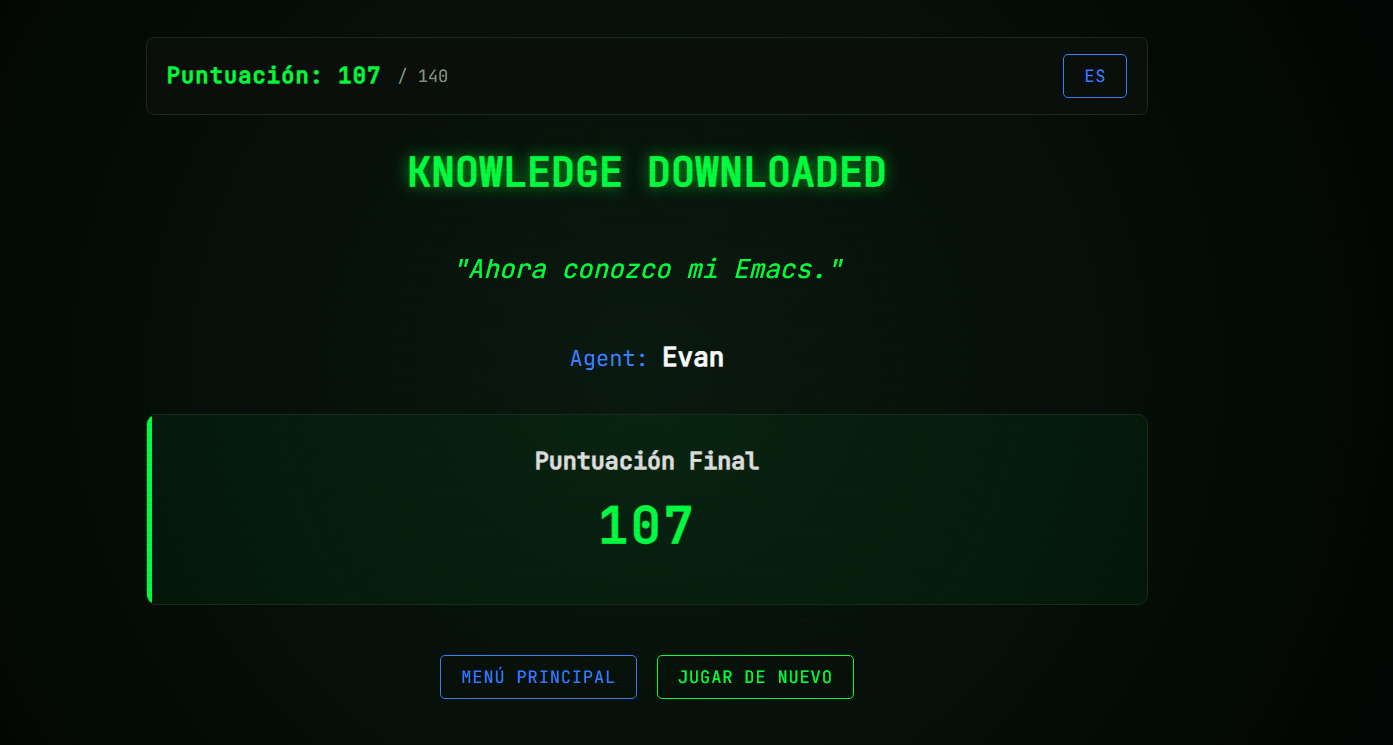
\includegraphics[width=.9\linewidth]{./EvanImagen.jpg}
\end{center}
\begin{center}
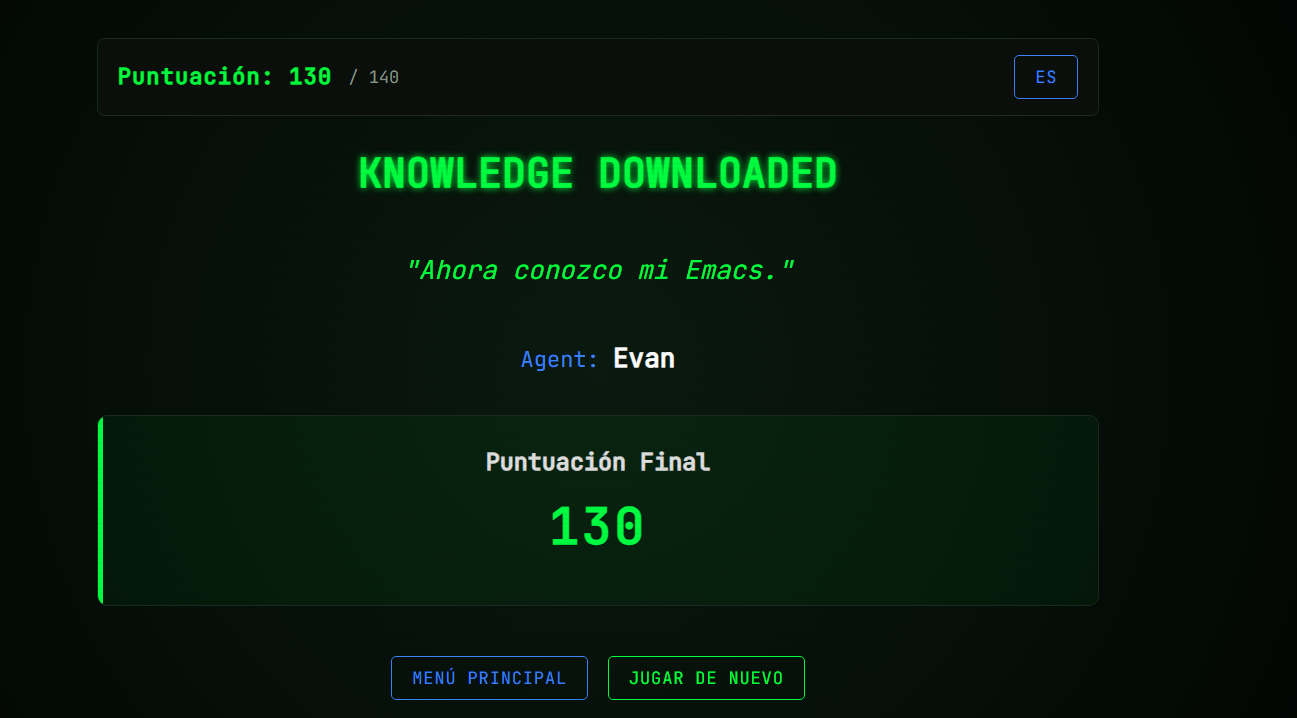
\includegraphics[width=.9\linewidth]{./EvanImagen2.png}
\end{center}
\begin{center}
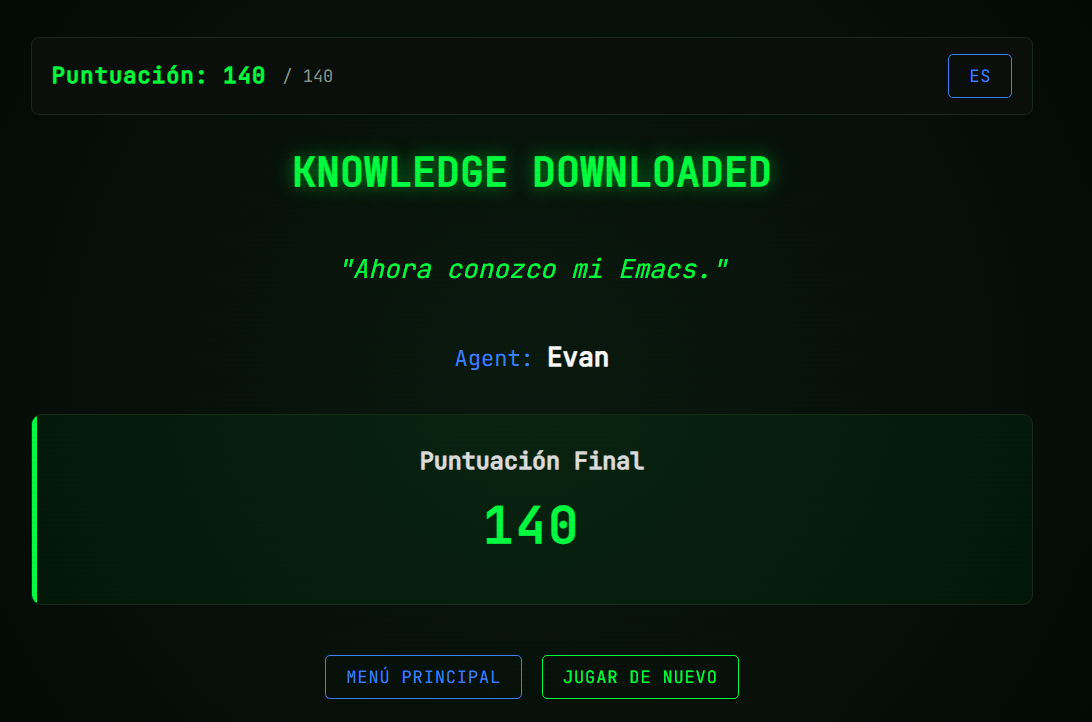
\includegraphics[width=.9\linewidth]{./EvanImagen3.png}
\end{center}


Estudiante B: Endara Sebastian
\begin{center}
\begin{tabular}{rr}
\hline
iteración & Puntaje\\[0pt]
\hline
1 & 140\\[0pt]
2 & 130\\[0pt]
3 & 130\\[0pt]
\hline
\end{tabular}
\end{center}

\begin{center}
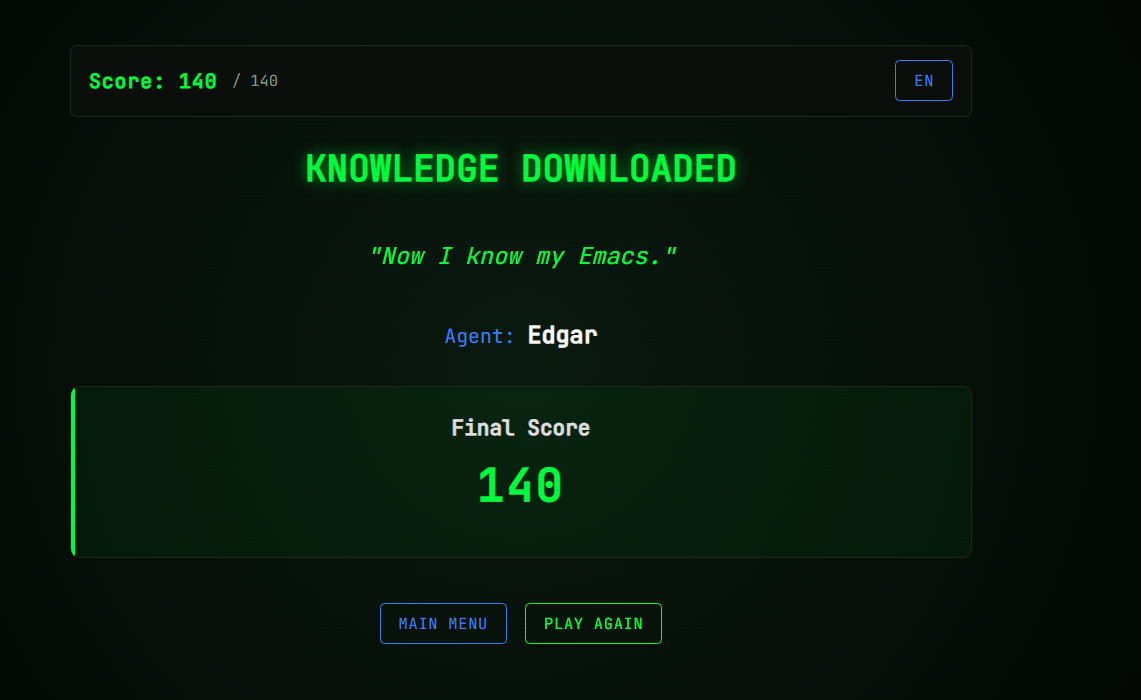
\includegraphics[width=.9\linewidth]{./ImagenesSebastian/EndaraSebastian1.png}
\end{center}
\begin{center}
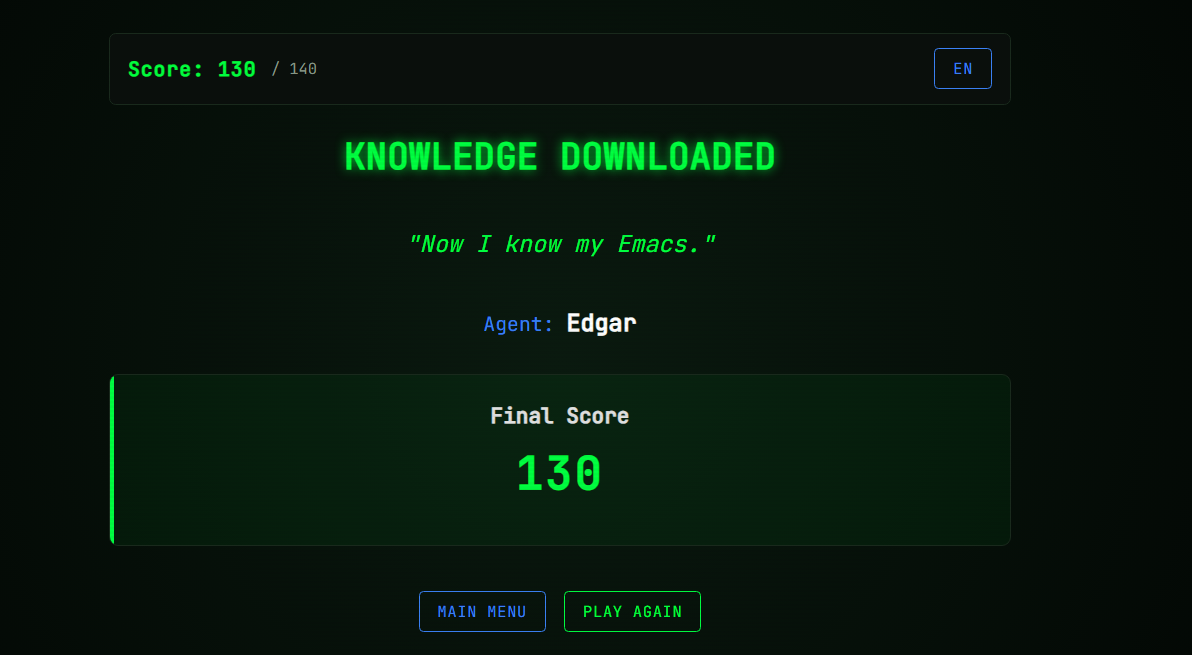
\includegraphics[width=.9\linewidth]{./ImagenesSebastian/EndaraSebastian2.png}
\end{center}
\begin{center}
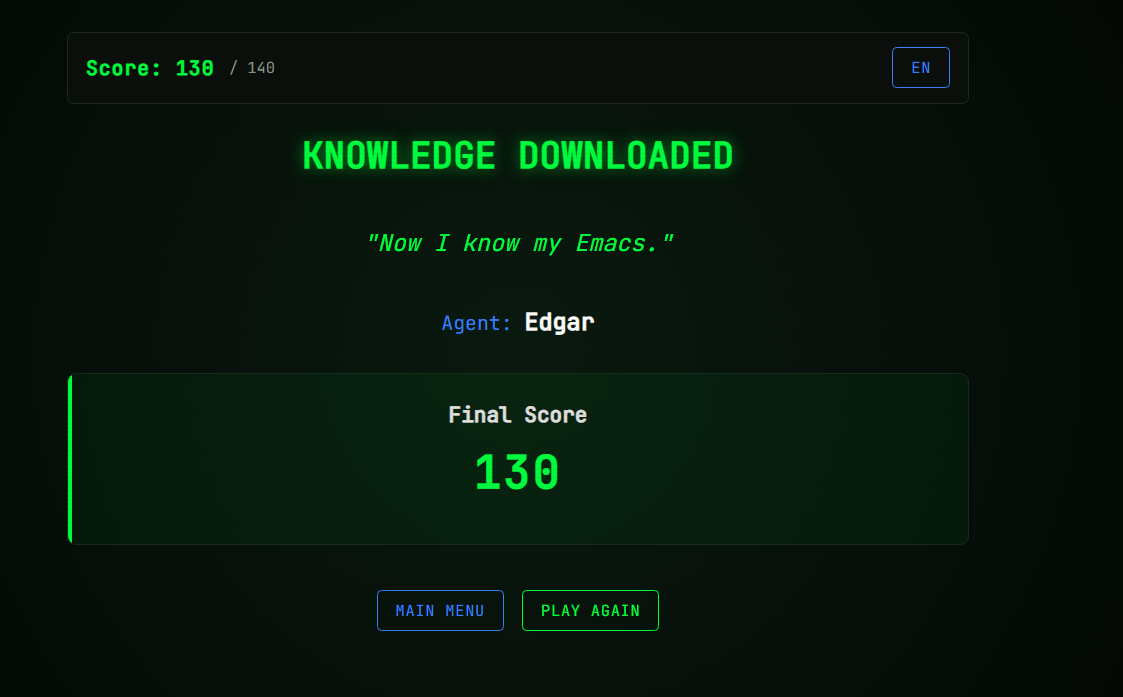
\includegraphics[width=.9\linewidth]{./ImagenesSebastian/EndaraSebastian3.png}
\end{center}

Estudiante C: Joset Muela
\begin{center}
\begin{tabular}{rr}
\hline
iteración & Puntaje\\[0pt]
\hline
1 & 96\\[0pt]
2 & 126\\[0pt]
3 & 120\\[0pt]
\hline
\end{tabular}
\end{center}


\begin{center}
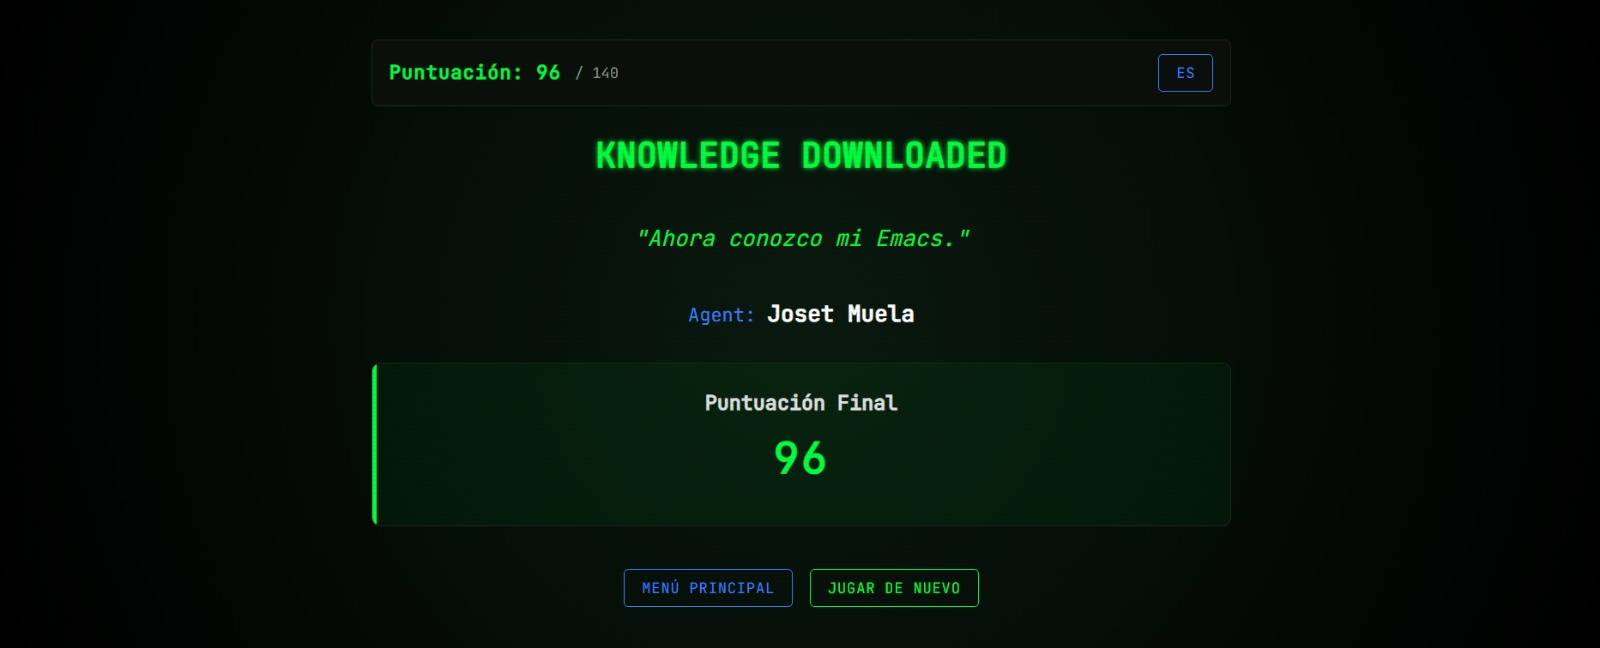
\includegraphics[width=.9\linewidth]{./ImagenesJoset/JosetImagen.png}
\end{center}
\begin{center}
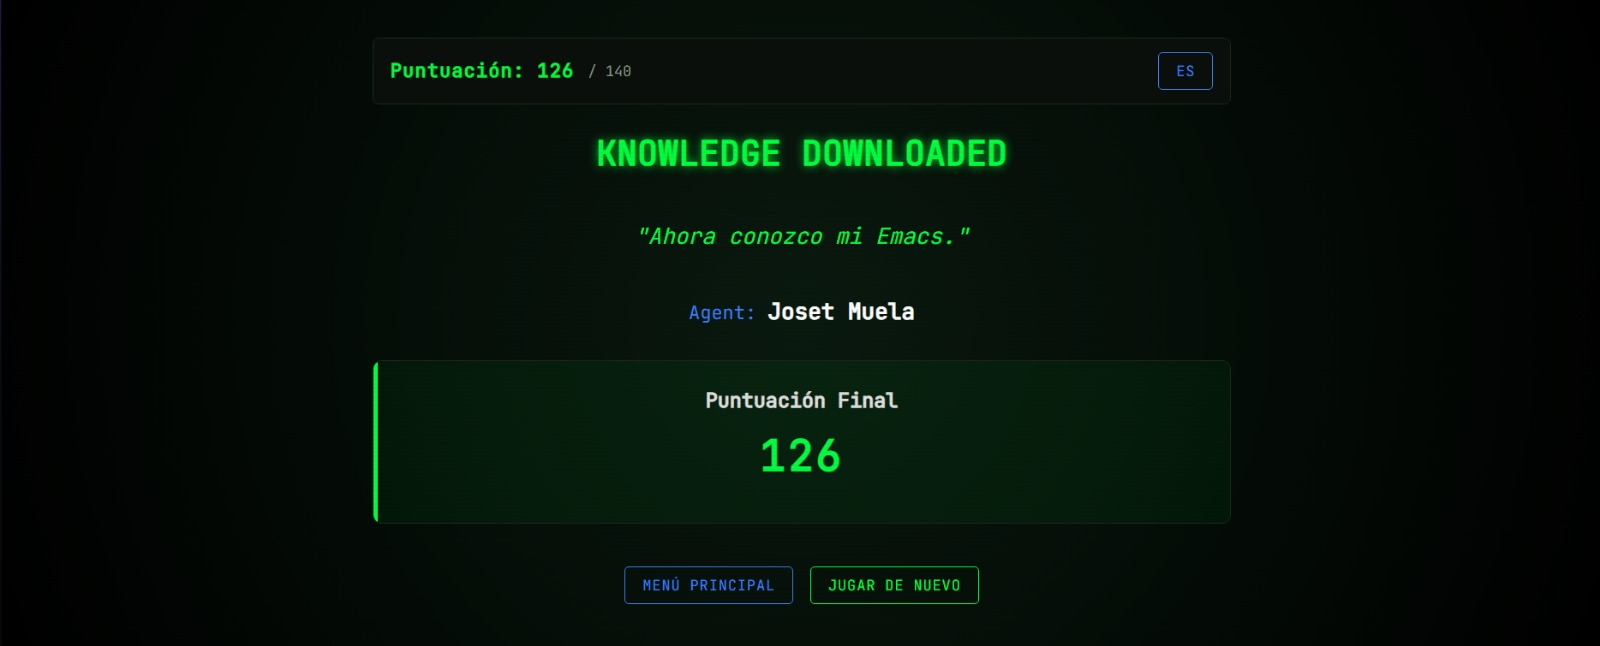
\includegraphics[width=.9\linewidth]{./ImagenesJoset/JosetImagen2.png}
\end{center}
\begin{center}
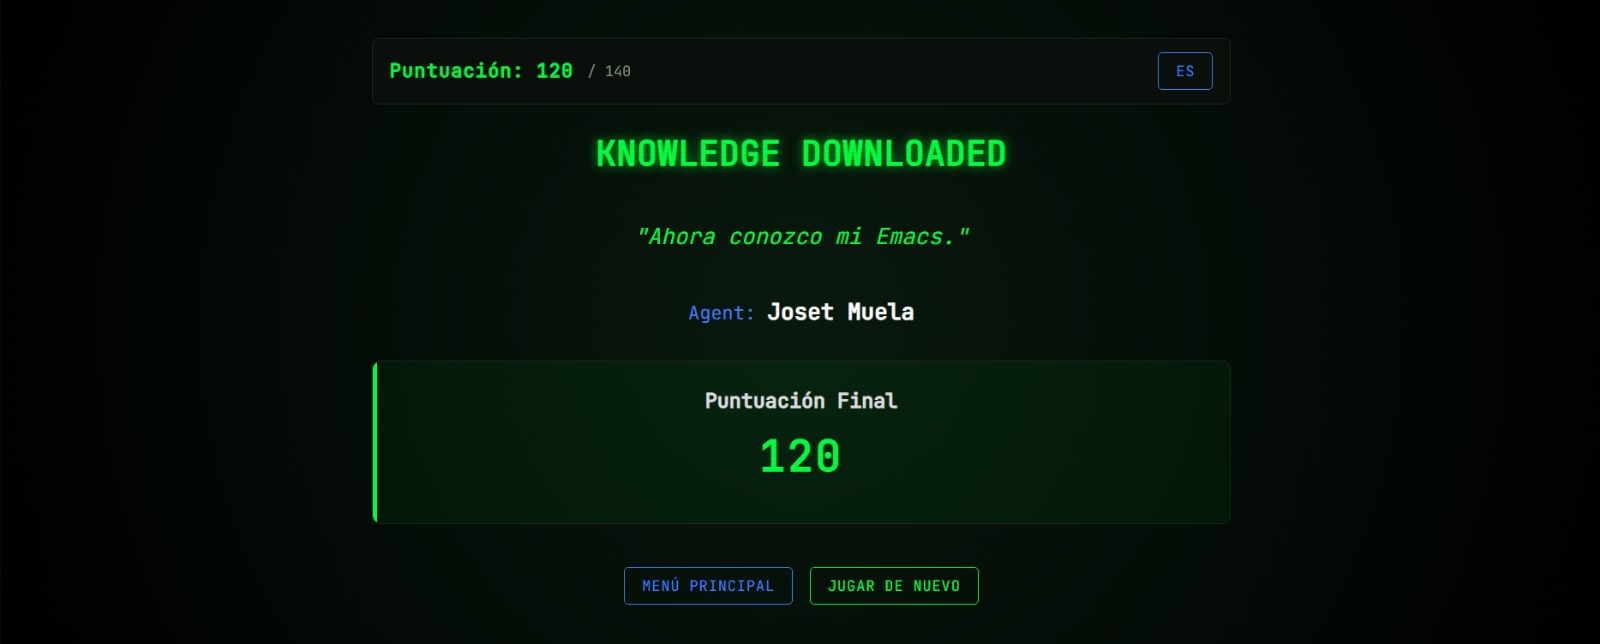
\includegraphics[width=.9\linewidth]{./ImagenesJoset/JosetImagen3.png}
\end{center}



Estudiante D: Karen Suarez
\begin{center}
\begin{tabular}{rr}
\hline
iteración & Puntaje\\[0pt]
\hline
1 & 77\\[0pt]
2 & 130\\[0pt]
3 & 130\\[0pt]
\hline
\end{tabular}
\end{center}

\begin{center}
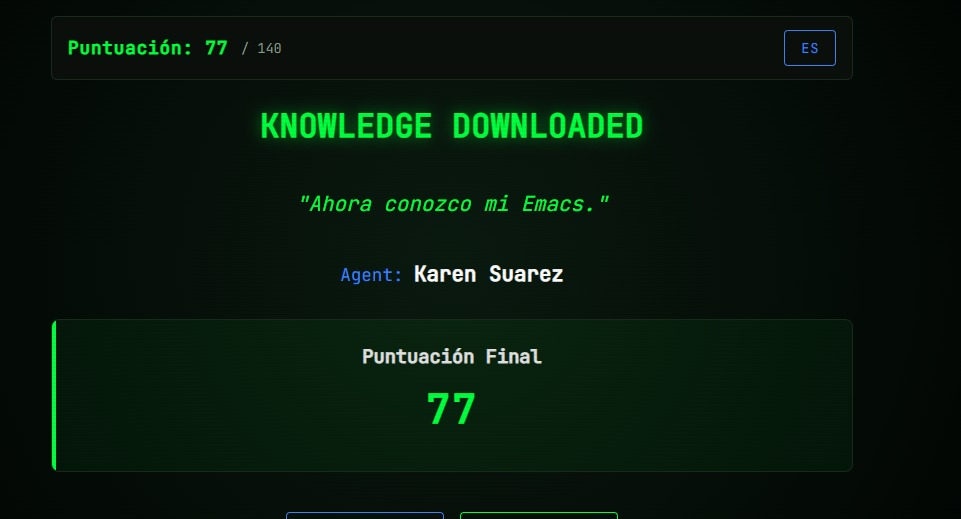
\includegraphics[width=.9\linewidth]{./KarenImagen.jpeg}
\end{center}
\begin{center}
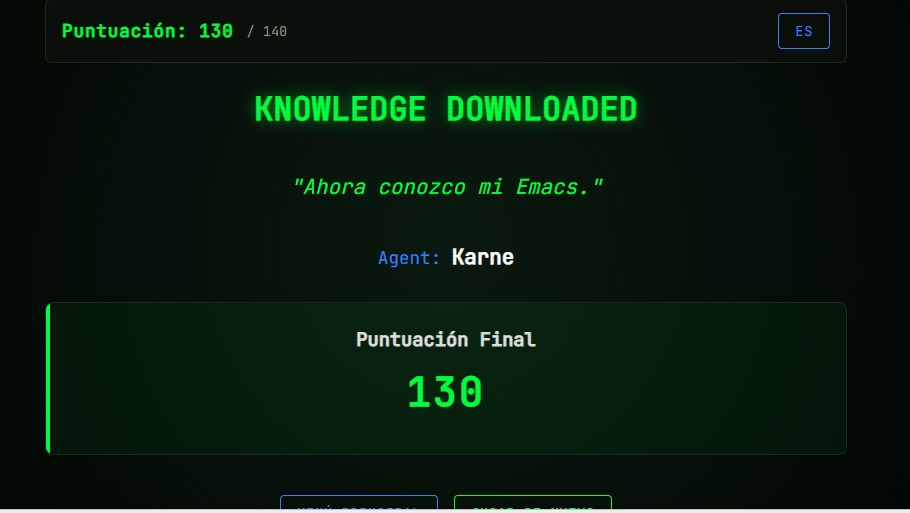
\includegraphics[width=.9\linewidth]{./karen.jpeg}
\end{center}
\begin{center}
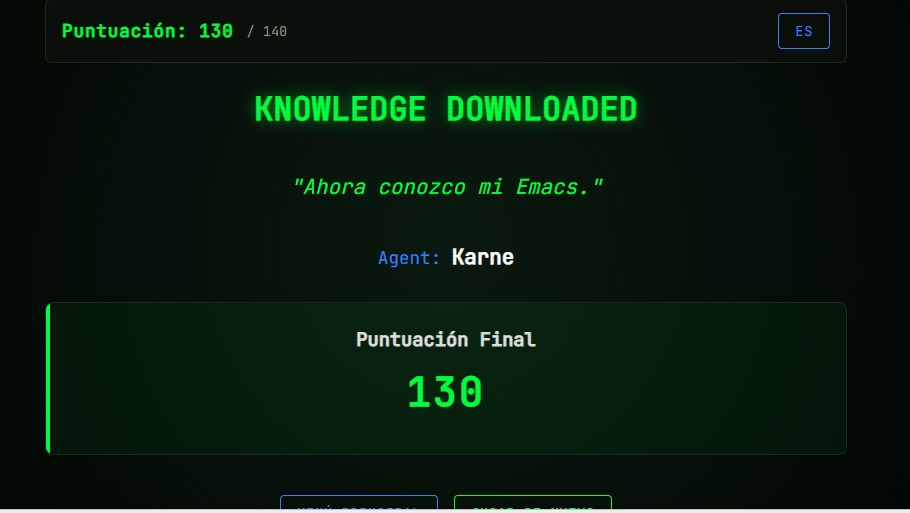
\includegraphics[width=.9\linewidth]{./karen.jpeg}
\end{center}

\subsection{Usando Emacs para tener Ayuda sobre Emacs}
\label{sec:org90b39dd}
¿Qué comandos le resultan más fáciles de usar y cuáles le son más
extraños? Identifique 4 comandos que le sean fáciles y 4 que le
resulten complicados. Revise qué dice la ayuda de Emacs sobre cada
comando y escriba en sus palabras el para qué sirve.

Para consultar lo que hace un comando ejecute:
\begin{enumerate}
\item \texttt{C-h k}
\item Emacs le preguntara cuál es la combinación de la que requiere
ayuda. Presione las teclas del comando. Por ejemplo, \texttt{C-x C-f}
\item Emacs abrirá un nuevo buffer con la descripción del comando.
\item Cambie al buffer de la ayuda con \texttt{C-x o}
\item Seleccione el primer parrafo de ayuda ubicando el cursor al inicio
del parrafo y activando la marcación de texto con
\texttt{C-SPC}. Seleccione avanzando por palabras \texttt{M-f} o directamente
toda la linea \texttt{C-e}
\item Una vez seleccionado, copie el texto con \texttt{M-w}.
\item Regrese al buffer anterior con \texttt{C-x o}.
\item Pegue el texto en <Pegar lo que dice el\ldots{}> con \texttt{C-y}
\end{enumerate}

\textbf{\textbf{Comandos Fáciles}}
\begin{enumerate}
\item \textbf{\textbf{Evan Matango:}} <C-f>. <Mover un espacio el cursor>
\item \textbf{\textbf{Estudiante B:}} <Poner el comando>. <Pegar lo que dice el primer párrafo de la ayuda>
\item \textbf{\textbf{Joset Muela:}}  <C-x C-s> <Guaradar un archivo>
\item \textbf{\textbf{Karen Suarez}} \texttt{C-x C-f}:C-x C-f runs the command find-file (found in global-map), which is an
\end{enumerate}
interactive native-compiled Lisp function in ‘files.el’. 

\textbf{\textbf{Comandos Difíciles}}
\begin{enumerate}
\item \textbf{\textbf{Estudiante A:}} <C-x k>. <Matar un buffer>
\item \textbf{\textbf{Estudiante B:}} <Poner el comando>. <Pegar lo que dice el primer párrafo de la ayuda>
\item \textbf{\textbf{Joset Muela:}}  <C-s> <Guaradar varios buffers>
\item \textbf{\textbf{Karen Suarez}} \texttt{C-x c-b}:C-x C-b runs the command list-buffers (found in global-map), which is
\end{enumerate}
an interactive native-compiled Lisp function in ‘buff-menu.el’


\section{Equipo de Trabajo}
\label{sec:org0f14257}
Complete la información de los integrantes de grupo e indique el líder
de grupo.

\begin{center}
\begin{tabular}{lll}
\hline
Nombre & email & Rol\\[0pt]
\hline
Evan Matango & evan.matango@epn.edu.ec & líder\\[0pt]
Edgar Endara & edgar.endara@epn.edu.ec & colaborador\\[0pt]
Karen Suarez & karen.suarez01@epn.edu.ec & colaborador\\[0pt]
Joset Muela & joset.muela@epn.edu.ec & colaborador\\[0pt]
\hline
\end{tabular}
\end{center}

\section{Verificación de Entregables [100\%]:}
\label{sec:org544a060}
Ejecute \texttt{C-c C-c} sobre los ítems de tarea según se hayan cumplido o
no. Si un ítem no pudo realizarse apunte en la siguiente sección las
razones al respecto.
\begin{itemize}
\item[{$\boxtimes$}] Verificación de configuración de entorno WSL y paquetes del curso.
\item[{$\boxtimes$}] Tutorial de Comandos Emacs realizado.
\item[{$\boxtimes$}] Captura de Imágenes y puntajes de Emacs Trainer App.
\item[{$\boxtimes$}] Usando Emacs para tener ayuda sobre Emacs
\item[{$\boxtimes$}] Verifique que estén los nombres de los integrantes del equipo e
identificado el líder.
\item[{$\boxtimes$}] Revisión de ortografía con \texttt{ispell} en el buffer
\item[{$\boxtimes$}] Generación de Archivo PDF \texttt{M-x org-latex-export-to-pdf}
\end{itemize}
\subsection{Problemas con la Tarea:}
\label{sec:org628c387}
\begin{itemize}
\item Tarea \(X_1\) no pudo completarse debido a
\item Tarea \(X_2\) no pudo completarse debido a
\end{itemize}
\end{document}
